\documentclass[svgnames,11pt]{standalone}
\usepackage[utf8]{inputenc}
\usepackage[T1]{fontenc}
\usepackage{csquotes}
\usepackage[english]{babel}
\usepackage{xcolor}
\usepackage{charter}
\usepackage{amsmath}
\usepackage{amssymb}
\usepackage[np,autolanguage]{numprint}
\newcommand{\outqt}[1]{{\textcolor{DarkOrange}{#1}}}
\newcommand{\inqt}[1]{{\textcolor{Blue}{#1}}}
\usepackage{tikz}
\usetikzlibrary{arrows,automata,calc}
\usetikzlibrary{arrows.meta}
\usetikzlibrary{decorations.pathreplacing}
\usetikzlibrary{backgrounds,shapes}
\tikzset{%
  show curve controls/.style={
    postaction={
      decoration={
        show path construction,
        curveto code={
          \draw [blue] 
            (\tikzinputsegmentfirst) -- (\tikzinputsegmentsupporta)
            (\tikzinputsegmentlast) -- (\tikzinputsegmentsupportb);
          \fill [red, opacity=0.5] 
            (\tikzinputsegmentsupporta) circle [radius=.25ex]
            (\tikzinputsegmentsupportb) circle [radius=.25ex];
        }
      },
      decorate
}}}
\tikzstyle{vertex}=[draw,circle,black,inner sep=2pt]
\tikzstyle{edge}=[line width=1.3pt,color=Black]
\tikzstyle{rare}=[fill=black,text=white]
\tikzstyle{medium}=[fill=black!15!white]


\begin{document}
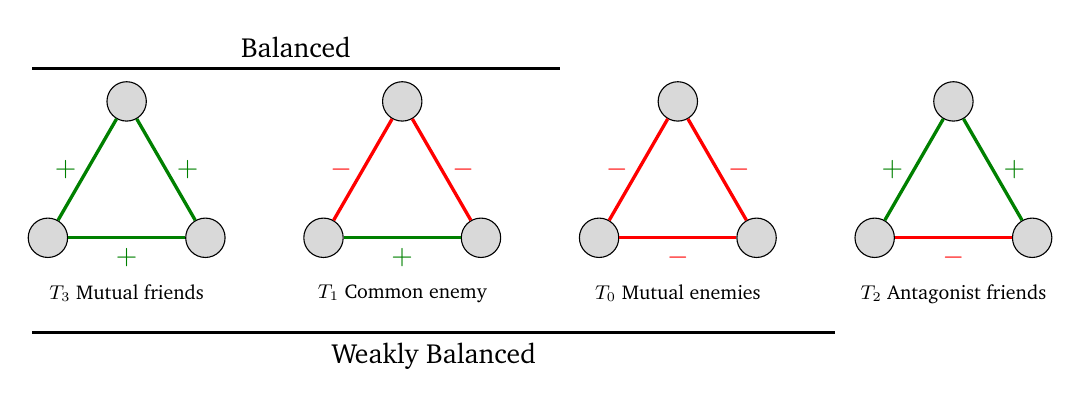
\begin{tikzpicture}[auto,vertex/.append style={minimum width=5mm},
  edge/.append style={line width=1.2pt,color=Black}]

  \node[vertex,medium,] (t11) at (0,0) {};
  \node[vertex,medium,] (t12) at (2,0) {};
  \node[vertex,medium,] (t13) at (1, 1.732) {};
  \draw[edge,Green] (t11) -- node[below] {$+$} (t12);
  \draw[edge,Green] (t11) -- node[left] {$+$} (t13);
  \draw[edge,Green] (t12) -- node[right] {$+$} (t13);
  \node[anchor=north,font=\small,scale=.8] (t1) at (1, -.5) {$T_3$ Mutual friends};

  \node[vertex,medium,] (t21) at (3.5,0) {};
  \node[vertex,medium,] (t22) at (5.5,0) {};
  \node[vertex,medium,] (t23) at (4.5, 1.732) {};
  \draw[edge,Green] (t21) -- node[below] {$+$} (t22);
  \draw[edge,Red] (t21) -- node[left] {$-$} (t23);
  \draw[edge,Red] (t22) -- node[right] {$-$} (t23);
  \node[anchor=north,font=\small,scale=.8] (t1) at (4.5, -.5) {$T_1$ Common enemy};

  \draw[edge,black,very thick] (-.20, 2.15) -- node[] {Balanced} (6.5, 2.15);

  \node[vertex,medium,] (t31) at (7,0) {};
  \node[vertex,medium,] (t32) at (9,0) {};
  \node[vertex,medium,] (t33) at (8, 1.732) {};
  \draw[edge,Red] (t31) -- node[below] {$-$} (t32);
  \draw[edge,Red] (t31) -- node[left] {$-$} (t33);
  \draw[edge,Red] (t32) -- node[right] {$-$} (t33);
  \node[anchor=north,font=\small,scale=.8] (t1) at (8, -.5) {$T_0$ Mutual enemies};

  \node[vertex,medium,] (t41) at (10.5,0) {};
  \node[vertex,medium,] (t42) at (12.5,0) {};
  \node[vertex,medium,] (t43) at (11.5, 1.732) {};
  \draw[edge,Red] (t41) -- node[below] {$-$} (t42);
  \draw[edge,Green] (t41) -- node[left] {$+$} (t43);
  \draw[edge,Green] (t42) -- node[right] {$+$} (t43);
  \node[anchor=north,font=\small,scale=.8] (t1) at (11.5, -.5) {$T_2$ Antagonist friends};
  \draw[edge,black,very thick,below] (-.20, -1.2) -- node[] {Weakly Balanced} (10, -1.2);
\end{tikzpicture}
\end{document}
